\documentclass[border=3pt]{standalone}
\usepackage{mathptmx}
\usepackage{tikz}
\usetikzlibrary{arrows.meta,fit,backgrounds,calc}
\begin{document}
\footnotesize % 8 pt: smallest text size allowed by the journal
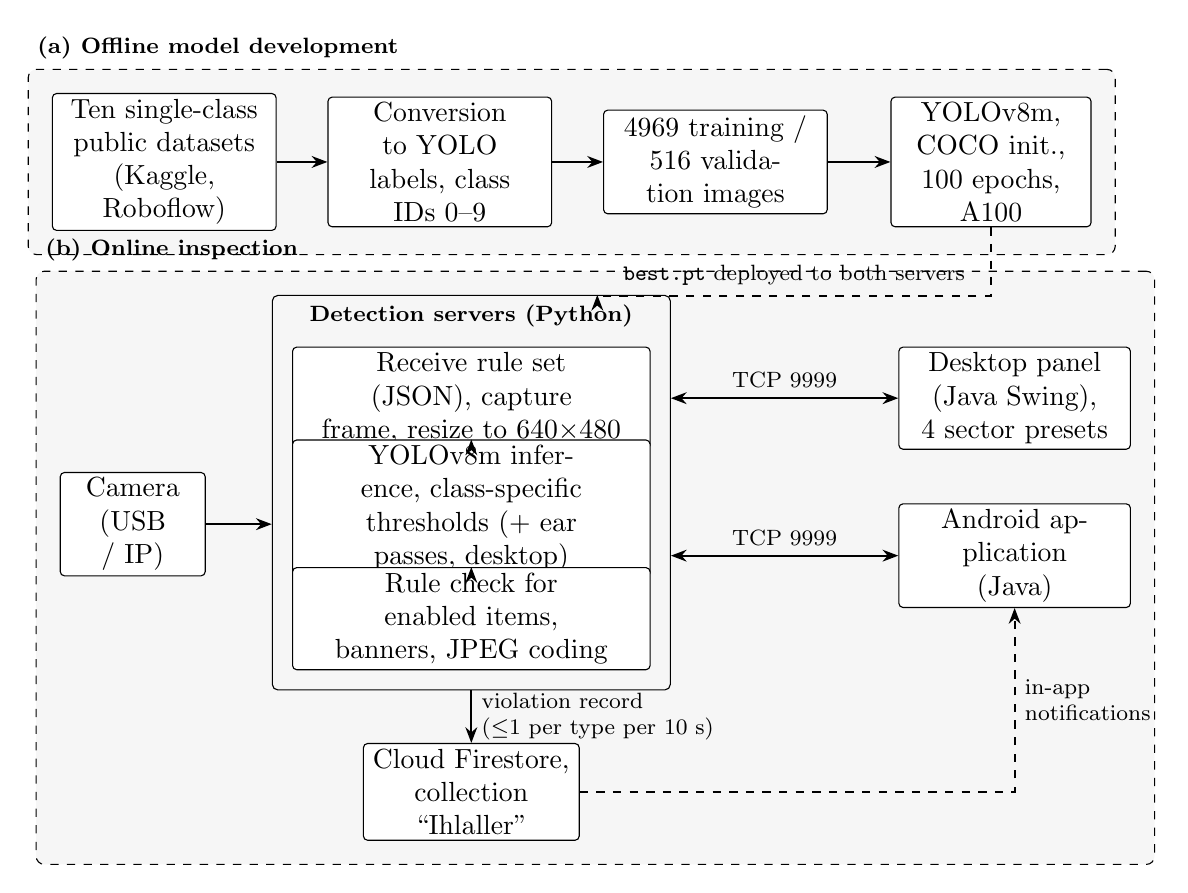
\begin{tikzpicture}[x=1mm,y=1mm,
  box/.style={draw, rounded corners=1.5pt, align=center, fill=white, inner sep=2pt, minimum height=11mm},
  grp/.style={draw, dashed, rounded corners=3pt, inner sep=3mm},
  arr/.style={-{Stealth[length=2mm]}, thick},
  darr/.style={{Stealth[length=2mm]}-{Stealth[length=2mm]}, thick},
]
% ---------------- (a) offline model development ----------------
\node[box, text width=27mm] (data)  at (15,0)  {Ten single-class\\public datasets\\(Kaggle, Roboflow)};
\node[box, text width=27mm] (conv)  at (50,0)  {Conversion to YOLO\\labels, class IDs 0--9};
\node[box, text width=27mm] (split) at (85,0)  {4969 training /\\516 validation images};
\node[box, text width=24mm] (train) at (120,0) {YOLOv8m, COCO init.,\\100 epochs, A100};
\draw[arr] (data) -- (conv);
\draw[arr] (conv) -- (split);
\draw[arr] (split) -- (train);
\begin{scope}[on background layer]
\node[grp, fill=gray!7, fit=(data)(train)] (g1) {};
\end{scope}
\node[anchor=south west, font=\footnotesize\bfseries] at (g1.north west) {(a) Offline model development};

% ---------------- (b) online inspection ----------------
\node[box, text width=17mm] (cam) at (11,-46) {Camera\\(USB / IP)};

\node[box, text width=44mm, minimum height=8mm] (s1) at (54,-30) {Receive rule set (JSON), capture\\frame, resize to 640$\times$480};
\node[box, text width=44mm, minimum height=8mm] (s2) at (54,-44) {YOLOv8m inference, class-specific\\thresholds (+ ear passes, desktop)};
\node[box, text width=44mm, minimum height=8mm] (s3) at (54,-58) {Rule check for enabled items,\\banners, JPEG coding};
\draw[arr] (s1) -- (s2);
\draw[arr] (s2) -- (s3);
\node[draw, rounded corners=2pt, inner sep=2.5mm, fit=(s1)(s3), yshift=2mm, inner ysep=4.5mm] (srv) {};
\node[anchor=north, font=\footnotesize\bfseries] at (srv.north) {Detection servers (Python)};
\draw[arr] (cam) -- (cam -| srv.west);
\coordinate (wx) at (70,0);
\draw[arr, dashed] (train.south) |- (70,-17) node[pos=0.75, above, font=\footnotesize]{\texttt{best.pt} deployed to both servers} -- (wx |- srv.north);

\node[box, text width=28mm] (desk) at (123,-30) {Desktop panel\\(Java Swing),\\4 sector presets};
\node[box, text width=28mm] (mob)  at (123,-50) {Android application\\(Java)};
\node[box, text width=26mm] (fb)   at (54,-80) {Cloud Firestore,\\collection ``Ihlaller''};
\draw[darr] (desk.west -| srv.east) -- node[above, font=\footnotesize]{TCP 9999} (desk.west);
\draw[darr] (mob.west -| srv.east) -- node[above, font=\footnotesize]{TCP 9999} (mob.west);
\draw[arr] (srv.south) -- node[right, font=\footnotesize, align=left]{violation record\\($\leq$1 per type per 10 s)} (fb.north);
\draw[arr, dashed] (fb.east) -| node[pos=0.75, right, font=\footnotesize, align=left]{in-app\\notifications} (mob.south);

\begin{scope}[on background layer]
\node[grp, fill=gray!7, fit=(cam)(srv)(desk)(fb)(mob)] (g2) {};
\end{scope}
\node[anchor=south west, font=\footnotesize\bfseries] at (g2.north west) {(b) Online inspection};
\end{tikzpicture}
\end{document}
